\chapter{Bezkonfliktné replikovateľné dátové typy}

\label{kap:cdrt} % id kapitoly pre prikaz ref

% TODO: definicie
% vymysli termonologiu pre zdroj/repliku
% hostitelia - entity zdielajuce zdroj ine pristupujuce k zdroju

Súbežné úpravy inštancie jedného zdroja bez koordinácie medzi jednotlivými hostiteľskými
počítačmi môže viesť k nekonzistentosti medzi zdrojmi, ktoré vo všeobecnosti nie je možné
vyriešiť. Riešenie konzistentnosti v takýchto prípadoch vyžaduje vrátenie niektorch operácii.

V distribuovanom výpočte je konfliktný replikovaný dátový typ (CRDT) dátová štruktúra,
ktorá môže byť replikovaná vo viacerých počítačoch v sieti, pričom jednotlivé inštancie je možné
aktualizovať nezávisle a súbežne bez koordinácie medzi ostanými inštanciami a kde je vždy
matematicky možné vyriešiť nezrovnalosti, ktoré by mohli vyplynúť. Z toho vyplýva, že použitím
CRDT nemôže nastať situácia, kde by sme museli nejakú operáciu vrátiť. 

Koncept CRDT bol formálne definovaný v roku 2011 osobami
Marc Shapiro, Nuno Preguiça, Carlos Baquero a Marek Zawirski \cite{crdt_definition}.

\section{Typy CRDT}
V súčastnosti sú preskúmané 2 typy CRDT:
\begin{enumerate}
  \item CRDT založené na operáciách
  \item CRDT založené na stavoch
\end{enumerate}

\subsection{CRDT založené na operáciách}
CRDT založené na operáciách sú označované ako komutatívne replikované dátové typy alebo 
\textit{CmRDT}. CmRDT menia zdroj vysielaním iba operácie, ktoré sa potom aplikujú lokálne
u všetkých, ktorý zdroj zdieľajú. Operácie musia byť komutatívne, avšak nemusia 
byť idempotentné. Je preto nutné zaručiť idempotenciu pomocou vhodnej implementácie
komunikácie (správa musí byť vyslaná práve raz). 
Jednoduchým príkladom, kde je vhodné použiť CmRDT je napríklad aktualizovanie počtu zdieľaní
príspevkov na sociálnych sieťach, kde sa server vie postarať o idempotentnosť. 

\subsection{CRDT založené na stavoch}
CRDT založené na stavoch sa nazývajú konvergentné replikované dátové typy alebo \textit{CvRDT}.
Na rozdiel od CmRDT posielajú celý svoj stav, kde stavy sa potom zlučujú funkciou,
ktorá musí byť komutatívna, asociatívna a idempotentná.

Posielanie celého stavu, nie je vždy optimálne. Častokrát stačí posielať zmeny, ktoré sa na zdroji
uskutočňujú. Takéto CRDT označujeme ako \textit{Delta CRDTs}

\section{Princíp fungovania CRDT}
CRDT funguje tak, že každý znak v dokumente sa prerobí do objektu so špecifickými vlastnosťami:
\begin{enumerate}
  \label{def_pozicie}
  % TODO: change 'znak' to 'atom'
  \item znak, ktorý objekt predstavuje
  \item relatívna pozícia tohto znaku
  \item množina pozícií musí tvoriť úplné usporiadanie
  \item priestor tvorený množinou pozícií musí byť hustý
\end{enumerate}
Vzhľadom na to, že každý z týchto objektov je jedinečný a môže byť identifikovaný
týmito vlastnosťami, môžeme zabrániť vloženiu alebo vymazaniu znakov viac ako raz.
To umožňuje komutativitu a idempotenciu. Nevýhodou tohto prístupu je veľké množstvo metaúdajov.
Tým sa zvyšuje spotreba pamäte aplikácie.

Zaujímavým aspektom CRDT, ktorý ho odlišuje od OT, sú relatívne pozície znakov. Tieto pozície majú
nasledovné vlastnosti:
\begin{enumerate}
  \item žiadne 2 CRDT objekty nemajú rovnakú pozíciu
  \item pozícia nejakého objektu sa nidky nezmení
  \item ak 2 CRDT objekty A a B operujú na tej istej pozícii v dokumente a objekt A
  nastane skôr než B, tak relatívna pozícia A musí byť menšia ako B.
\end{enumerate}
Vytvorenie takýchto pozícií je celkom jednduché.
Znaky si môžeme predstaviť ako vrcholy na strome, kde každý znak má väčsie číslo ako znak pred
ním, no menšie ako znak po ňom. Pozície môžu vyzerať zhruba nasledovne:

\begin{figure}[H]
\centerline{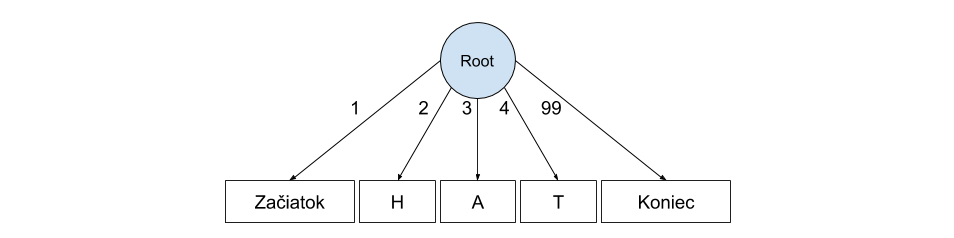
\includegraphics[width=0.6\textwidth]{images/relativne_pozicie1}}
%popis obrazku
\caption[Relatívne pozície znakov]{Relatívne pozície znakov}
%id obrazku, pomocou ktoreho sa budeme na obrazok odvolavat
\label{obr:relativne}
\end{figure}

Pridanie znaku potom funguje veľmi jednoducho. Nájdeme v strome vrcholy medzi ktoré
chceme pridať ďalší znak a ako pozíciu mu dáme priemer relatívnych pozícií daných
vrcholov. Napríklad:
\begin{figure}[H]
\centerline{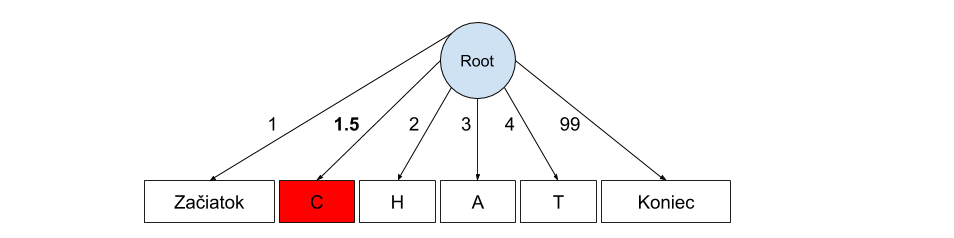
\includegraphics[width=0.6\textwidth]{images/relativne_pozicie2}}
%popis obrazku
\caption[Pridanie relatívnej pozície znakov]{Pridanie relatívnej pozície znakov}
%id obrazku, pomocou ktoreho sa budeme na obrazok odvolavat
\label{obr:relativne_pridanie}
\end{figure}

\begin{flushleft}\textbf {Komutativita a idempotentnosť CRDT}\end{flushleft}
Ak predpokladáme, že pozície spĺňajú podmienky z \ref{def_pozicie}, tak CRDT objekty sú
komutatívne a idempotentné. 

Keďže všetky relatívne pozície sú unikátne, tak nezáleží na poradí, v ktorom vykonávame dané operácie,
teda CRDT sú naozaj komutatívne.

Idempotencia je daná tým, že ak chceme do dokumentu pridať znak s najekou relatívnou pozíciou, a tá
sa tam už nachádza, tak opätovné pridanie už nič neurobí. Ak naopak sa snažíme vymazať niečo na
pozícii, ktorá sa v dokumente už nenachádza, tak vieme, že uz vymazaná bola. Obe operácie teda
zachovávajú idempotentnosť.
\cite{nuno_preguica}

\section{Použitie v praxi}
Aplikácie CRDT sa dajú nájsť nielen v oblasti kolaboratívnych editorov, ale na mnohých ďalších
miestach. Príkladom sú napríklad databáza \textit{Redis}, \textit{SoundClound} alebo NoSQL 
%TODO: definuj NoSQL 
dátové úložisko \textit{Riak}, ktoré sa používa na vnútorný chatovací systém v hre 
\textit{League of Legends}.
\cite{crdt_wiki}

% TODO: obrazky
